\documentclass[12pt]{article}
\usepackage[a4paper, margin=0.8in]{geometry}

\usepackage{amsfonts, amsmath, amsthm, amssymb}
\usepackage[utf8]{inputenc}
\usepackage[english]{babel}
\usepackage[T1]{fontenc}
\usepackage{color}
\usepackage{listings}
\usepackage{graphicx}
\usepackage{indentfirst}
\usepackage[document]{ragged2e}
\usepackage{hyperref}
\usepackage{graphicx,xcolor}
\usepackage{svg}

\usepackage{amsmath}
\usepackage{natbib}
\usepackage{graphicx}
\usepackage{algorithm}
\usepackage{algorithmic}
\usepackage{float}
\usepackage{pgfplots}

\usepackage{caption}
\usepackage{listings}
\usepackage{xcolor}
 
\definecolor{codegreen}{rgb}{0,0.6,0}
\definecolor{codegray}{rgb}{0.5,0.5,0.5}
\definecolor{codepurple}{rgb}{0.58,0,0.82}
\definecolor{backcolour}{rgb}{0.95,0.95,0.92}
 
\lstdefinestyle{pythonStyle}{
    backgroundcolor=\color{backcolour},   
    commentstyle=\color{codegreen},
    keywordstyle=\color{magenta},
    numberstyle=\tiny\color{codegray},
    stringstyle=\color{codepurple},
    basicstyle=\ttfamily\footnotesize,
    breakatwhitespace=false,         
    breaklines=true,                 
    captionpos=b,                    
    keepspaces=true,                 
    numbers=left,                    
    numbersep=5pt,                  
    showspaces=false,                
    showstringspaces=false,
    showtabs=false,                  
    tabsize=2
}
\lstset{style=pythonStyle}

\newcommand\underrel[2]{\mathrel{\mathop{#2}\limits_{#1}}}




\begin{document}


\thispagestyle{empty}
\noindent\fbox{%
    \parbox{\textwidth}{%
        \center{\Large{Automatic differentiation}}
        \center{}
    }%
}
\justify

\tableofcontents


%%%%%%%%%%%%%%%%%%%%%%%%%%%%%%%%%%%%%%%%%%%%%%%%%%%%%%%%%%%%%%%%
%
%               TYPES OF DIFFERENTIATION
%
%%%%%%%%%%%%%%%%%%%%%%%%%%%%%%%%%%%%%%%%%%%%%%%%%%%%%%%%%%%%%%%%


\section*{Types of differentiation}

There are 3 methods of computing the derivative of a function evaluated at a specific point :

\begin{itemize}
\item Symbolic
\item Numerical
\item Automatic Differentiation (AD)
\end{itemize}


%%%%%%%%%%%%%%%%%%%%%%%%%%%%%%%%%%%%%%%%%%%%%%%%%%%%%%%%%%%%%%%%
%
%               SYMBOLIC DIFFERENTIATION
%
%%%%%%%%%%%%%%%%%%%%%%%%%%%%%%%%%%%%%%%%%%%%%%%%%%%%%%%%%%%%%%%%

\section{Symbolic differentiation}


It's the same as we do when computing manually the derivative of a function to get its value at a specific point. We take the input expression and apply rules of differentiation such as :

\begin{itemize}
\item $$ \frac{d}{dx}(f \times g) = \frac{d}{dx}f \times g + \frac{d}{dx}g \times f $$
\item $$ \frac{d\sin}{dx} = \cos $$
\item $$\frac{d}{dx}\frac{f}{g} = \frac{ g \times \frac{d}{dx}f - f \times \frac{d}{dx}g }{g^2}$$
\end{itemize}

Symbolic computing takes in input an expression and then only use its symbolic representation for each operation (in other words, the program keeps using `x` instead of the value of `x` for calculation). It's really helpful to get the exact form of a result since there cannot be any error of rounding or floating precision because no value is used at all.

For example, with Python the symbolic differentiation works as following :

\begin{lstlisting}[language=Python, escapeinside={(*}{*)}, numbers=none]
import sympy as sym

x = sym.Symbol('x') # declare x as a symbolic variable
t = sym.Symbol('t')

f = sym.sin(x*(t**2)) # definition of the expression
f_prime = f.diff(x) # compute the symbolic form of the derivative (first order, aka df/dx) with respect to x
\end{lstlisting}

Then

\begin{lstlisting}[language=Python, escapeinside={(*}{*)}, numbers=none]
print(f)
>> sin(t**2*x)
print(f_prime)
>> t**2*cos(t**2*x)
\end{lstlisting}

To get the value of the derivative at one point (by replacing the symbolic representations of the variables with their respective values) :

\begin{lstlisting}[language=Python, escapeinside={(*}{*)}, numbers=none]
# Evaluate the derivative of f with x=2, t=3
f_prime.evalf(subs={x: 2, t:3})
>> 5.94285037419672
\end{lstlisting}

The main issue with symbolic computing is that it needs to expand each expression to get its reduced form. For example $(x+y+z)^3$ expands to $x^2+2xy+y^2+2xz+2yz+z^2$. And that expansion, then simplification has a prohibitive cost for longer expression.

And because of that overhead and time consuming method, it's not the usual way to compute derivatives.

%%%%%%%%%%%%%%%%%%%%%%%%%%%%%%%%%%%%%%%%%%%%%%%%%%%%%%%%%%%%%%%%
%
%               NUMERICAL DIFFERENTIATION
%
%%%%%%%%%%%%%%%%%%%%%%%%%%%%%%%%%%%%%%%%%%%%%%%%%%%%%%%%%%%%%%%%


\section{Numerical differentiation}

It's the go to method for computing derivative in a simple and fast way. But it comes with a trade off : precision. Numerical differentiation approximates numerically the value of the derivative, but does not compute its exact value.

Let's dig into how does it work.

%%%%%%%%%%%%%%%%%%%%%%%%%%%%%%%%%%%%%%%%%%%%%%%%%%%%%%%%%%%%%%%%
\subsection{What is a derivative ?}

First of all, we need to understand how derivative is defined to understand numerical differentiation. 

%%%%%%%%%%%%%%%%%%%%%%%%%%%%%%%%%%%%%%%%%%%%%%%%%%%%%%%%%%%%%%%%
\subsubsection{Definition of a function}

A function describes a transformation/a relation from one set (in a mathematical sense) to another. For example, we could have a relation that gives the coordinates of an object in the 2D plan with respect to time $t$. At any time $t$ the object has for coordinate $(C_x(t), C_y(t))$ (usually coordinates are represented by $(x(t), y(t))$ but in order to mitigate any doubts from notations we made a distinction here). $C_x$ and $C_y$ are two functions :


\begin{itemize}
\item[]
$$
C_x: 
    \begin{cases}
        \mathbb{R} \rightarrow \mathbb{R} \\
        t \longmapsto C_x(t)
    \end{cases}
$$

\item[]
$$
C_y: 
    \begin{cases}
        \mathbb{R} \rightarrow \mathbb{R} \\
        t \longmapsto C_y(t)
    \end{cases}
$$
\end{itemize}



The two functions could have, for example, for graphical representation the following graphs : 


\begin{figure}[H]
 \centering
 \includesvg[width=1\columnwidth, svgpath = assets/images]{OnBrbQL6Yj.svg}
\end{figure}

Naturally, we want to superimpose the two graphs to see the evolution of the y coordinate with respect to the $x$ coordinate (after all , that the graph which really represent the motion of the object in the 2D plan). 

Let's define :
\begin{itemize}
    \item[] $X := \{{ C_x(t) | t \in Ker(C_x) \cap Ker(C_y) \}} = Im(C_x)$
    \item[] $Y := \{{ C_y(t) | t \in Ker(C_x) \cap Ker(C_y) \}} = Im(C_y)$
\end{itemize}

Note that since $C_x$ and $C_y$ have the same Kernel (because they share the same time sequence) :
$$
Ker(C_x) \cap Ker(C_y) = Ker(C_x) = Ker(C_y)
$$

Then, the corresponding composition function $C$ is :

$$
C: X \rightarrow Y
$$

where for $a \in X$, $f(a)=b \in Y$ with 

$$
\begin{cases}
t \in Ker(C_x) \cap Ker(C_y) \\
a = C_x(t) \\
b = C_y(t) \\
\end{cases}
$$
Note that $C$ is the function that map for the same moment in time $t$ the value of $C_x(t)$ to $C_y(t)$

\bigskip

$C$ can be written as :

$$
C:
\begin{cases}
X \rightarrow Y \\
a \mapsto C_y(C_x^{-1}(a))
\end{cases}
$$

With $C_x^{-1}$ the inverse image of $C_x$ by $X$

\begin{figure}[H]
 \centering
 \includesvg[width=0.7\columnwidth, svgpath = assets/images]{rQns64I4tv.svg}
\end{figure}

%%%%%%%%%%%%%%%%%%%%%%%%%%%%%%%%%%%%%%%%%%%%%%%%%%%%%%%%%%%%%%%%
\subsubsection{History of differentiation}

The notion of derivatives is not so old and find its origin in the field of Physics.
The question was : from a specific time $t_1$ where the object will be a few moments after ? In a graphical way, how to approximate the graph after the time $t_1$ (based on the knowledge of the previous points) ?

The main hypothesis which is natural is to consider that there is not so much changes if the two points are really really close, then we can approximate the graph between the two points as a straight line. And that is the foundation of differentiation.

Take a look at a potential graph of the function $C$. The goal is to find each quantity `...` (which could be different for each axis/dimension).

\begin{figure}[H]
 \centering
 \includesvg[width=0.7\columnwidth, svgpath = assets/images]{sQ6Rxqpqbe.svg}
\end{figure}

To simplify, let's define $x_i:=C_x(t_i)$ and $y_i:=C_y(t_i)$. Note that $:=$ means "equality is by definition".

In fact, it's not really about the proximity of the points chosen but the time elapsed to go from $P_1:=(C_x(t_1)=x_1, C(C_x(t_1))=C_y(t_1)=y_1)$ to $P2:=(C_x(t_2)=x_2, C(C_x(t_2))=C_y(t_2)=y_2) := (x_1+..., y_1+...)$, with $t_2 := t_1 + o$ where $o$ is really really really small time quantity. 

%%%%%%%%%%%%%%%%%%%%%%%%%%%%%%%%%%%%%%%%%%%%%%%%%%%%%%%%%%%%%%%%
\subsubsection{Notion of speed and velocity}

The first derivatives were used to explain the physical phenomena which intrinsically imply the evolution along time. That's why when we represent the motion of an object in the y-coordinate with respect to the x-coordinate there is another hidden axis : time.
\newline
A lot about the origin of derivative is based on things that are hard-wired to our daily experience of living.

%%%%%%%%%%%%%%%%%%%%%%%%%%%%%%%%%%%%%%%%%%%%%%%%%%%%%%%%%%%%%%%%

\paragraph{Some words about Time}


Time is the named of the concept that we need to explain the motion of objects. In fact, the correlation between time and movement of objects has been named motion.
We have an intrinsic understanding of time thanks to our body which has some \href{https://kids.frontiersin.org/articles/10.3389/frym.2019.00005}{clock proteins} which are  produced and broken down in a cycle that last 24h (which is called the circadian cycle). The only way for us to explain, to measure the motion of an object is \href{https://iep.utm.edu/aristotle-motion/\#H3}{time}. In fact, the simple fact to speak about motion and time is already a tautology.

The definition of time is just something that we can related to describe some phenomena without what we could not understand them. The motion of any object cannot be described without an evolution along what we call time. Without the notion of time, the graph of $C$ would have been a bunch of points that cannot be placed, cannot be ordered. It's because the graph of $C$ comes from the combination of the motion along two axis that need to be merged with respect to something shared/common between the two axis. At a specific moment, we can observe the position of an object as an image. At another moment, the position of the object has changed in the image. That difference of coordinates in the image is only explained because we can biologically observe an evolution from one of ours "sensors" that "measure time".

Later, what we can biologically feels has been more explicitly defined to have a standard definition. The actual \href{https://www.nist.gov/how-do-you-measure-it/how-do-we-measure-time}{definition of time} is given by the \href{https://en.wikipedia.org/wiki/International_Atomic_Time}{emission of radiation} from atoms that have a regular rate. Then this rate is adjusted to match what we know being 24h hours (which is approximately given by the clock proteins that have probably matched  the cycle of day/nigh in our planet).

\href{https://www.youtube.com/watch?v=EedRLTlOp20&ab_channel=Scilabus}{If time was a physical dimension} (a 4D space) then we may not need this concept anymore because we could literally see object evolving along that "time" dimension as we see objects if the 3D space. But in our vision of world there is something missing to \href{https://www.youtube.com/watch?v=NDYIdBMLQR0&ab_channel=argerichrichter1234}{explain motion}. And that's what time is trying to solve. As a comparison, a living being in a 2D world would need the concept of time to describe the third dimension that we have and that he's missing. For them, an object is described by the time needed to entirely see it and the shape of the projection of our 3D object in their 2D plan view (living in a 2D world means having a view in a 2D plan. It's the normal plan for them, but for us it's 2D relative to our 3D world).

\begin{figure}[H]
 \centering
 \includesvg[width=0.7\columnwidth, svgpath = assets/images]{1n6urRfqjL.svg}
 \caption*{Representation of the view of a living being in a 2D world vision}
\end{figure}
The time dimension is needed for them to understand the 3rd dimension of our 3D pen.

\bigskip

Time is useful to resolve problem without really being able to define it. And maybe there is some other concept that describe motion better, like other geometries better describe some problems in our world.

\paragraph{Speed and motion}

Speed is a central concept in derivative and it's built on top of the motion. The definition of speed is a pretty old concept. For example \href{http://classics.mit.edu/Aristotle/physics.7.vii.html}{\it The Physics} by Aristotle describes the notion of speed and velocity :
\begin{itemize}
    \item
\begin{quote}
[...] two things are of the same velocity if they occupy an equal time in accomplishing a certain equal amount of motion. [...] We may say, therefore, that things are of equal velocity in an equal time they traverse the same magnitude - {\it Book 7, part 4}
\end{quote}

    \item
\begin{quote}
 Then, A the movement have moved B a distance G in a time D, then in the same time the same force A will move 1/2B twice the distance G, and in 1/2D it will move 1/2B the whole distance for G: thus the rules of proportion will be observed - {\it Book 7, part 4}
\end{quote}
\end{itemize}


The speed is the amount of distance travelled with respect to the time elapsed. So why is it useful ? Because from a point $t_a$ in time if we want to know the distance traveled to another moment $t_b$ you just have to know the speed of the object at $t_a$(with the hypothesis that the speed at $t_a$ is representative of the average speed in $[t_a, t_b]$). The distance travelled is then $(t_b-t_a) \times speed|_{t_a}$.

This definition does not come from nowhere. It's coming because we have observed that an object at each point of the time has what we call speed/velocity which comes from the fact that the object is put in motion by a force (external or internal). 
Speed can be measured experimentally at "each" (at least at enough moments in time that we can no longer make a difference) points of time by taking some really small intervals of time ($\Delta_t$ really small) and measuring during that interval how much an object has moved.
Thus, the simple knowledge of that force (how much it's pushing the object and in what direction) gives us a pretty rule of proportion (with the hypothesis that the force is constant : it's pushing with the same amount of strength, and in the same direction). 

Since we assume that the initial force is representative of the average force between $t_a$ and $t_b$, then we can approximate the distance at $t_b$ only from the knowledge of the forces and position of the object (with its mass) at $t_a$.
In other words, it's strictly the same as drawing a straight line between two points to approximate the graph of a function between that two points. We just have to know how the line is oriented and when to stop it.

Of course this is not true in general : forces are not always constants and are usually not representative of the average speed. But it's quite true if the time elapsed between $t_a$ and $t_b$ is small enough. And experimental testing tends to comfort that hypothesis. 

\bigskip

This short recap of history is only present to bring to the light the nature of speed which is not a tool simply invented but which is intrinsically related to the Physics of our world. We observe that in some cases to push an object along the same distance (let say from point $A$ to $B$ in a straight line), we need to apply a force $F$ (let say a constant force) that will takes a specific time $\Delta_t$ to move. And we observe that we can move that same object, along the same distance half the time of the first experience, by applying the double of the force.
And to compare that two experiences, we need to compare how much the object has been moved at each moment, we need to compare a rate. Because some experiences could have different distance or different duration. So we need something that represents a ratio to be able to compare them at each point of the time no matter the initial parameters (distance, duration, ...). That ratio is the today well known : $\frac{\Delta_d}{\Delta_t}$ where $\Delta_d$ is the total distance between $A$ and $B$, and $\Delta_t$ is the time elapsed. That rate is then called speed.

Of course when the force is non constant, speed will change and the ratio $\frac{\Delta_d}{\Delta_t}$ can no longer be applied for the whole motion of the object because for certain moments/intervals of moments, this rate could be higher or lower than the previous or next moments. Then, we understand why we need to repeat the same operation for lot of points of the graph with really small time intervals. 

Being in the scope of mathematics the "small" is in fact a limit : if we need to do the operation for a lot of points of the graph to gain accuracy, in fact we can go on for infinity (because the small interval can always be split in smaller interval for continuous functions, at least in the usual space) and the only end is when we can have the speed of a single point (no more extremely small intervals that are representative of a specific point on the graph, just the speed for that single point at a single moment in time). This is what the limit represents.

By the way, what we have done for distance with respect to time (which give the speed) can also be done for its speed with respect to time which represents at each moment how much the speed changes (which is called acceleration).

\bigskip 

In conclusion :

\begin{quote}
    The speed is the instantaneous rate of change of the distance with respect to the time
\end{quote}

%%%%%%%%%%%%%%%%%%%%%%%%%%%%%%%%%%%%%%%%%%%%%%%%%%%%%%%%%%%%%%%%
\subsubsection{Derivative definition}


Going back to our initial problem, by knowing the speed of an object at a specific point, we then can determine form a specific point what will be its next position.

If we take a one dimensional example (our object is only moving along a line)


\begin{figure}[H]
 \centering
 \includesvg[width=1\columnwidth, svgpath = assets/images]{yQAOsqOt4J.svg}
\end{figure}


Then $(x_1+...) = x_1 + speed|_{t_1} \times o$ where $speed|_{t_1}$ is the speed of the object at the moment $t_1$ and $o$ that really small quantity ($o \neq 0$) in time. We take two moments in time really close and we suppose that all the forces and constraints remain the same during that really small change in time. Then we can apply a basic rule of proportion. Historically, the speed or \href{https://en.wikipedia.org/wiki/Velocity}{velocity} (the directional speed/the speed along a specific axis, along a specific degree of freedom of the object) is noted $\dot{x}$ (for the speed along the $x$ axis).


The, we can write $P_2$ as $(x_1 + \dot{x_1} \times o, y_1 + \dot{y_1} \times o)$. Note that $\dot{x_1} = \dot{C_x(x(t_1))} = speed|^x_{t_1}$ is the speed of the object along the $x$ axis at the time $t_1$. This is the notation used by Newton (see \href{http://www.sfu.ca/~rpyke/fluxions.pdf}{1}, \href{https://www.youtube.com/watch?v=i5TFXyI4UMM&ab_channel=Mathoma}{2}) when he first introduces his own version of derivatives. The quantities along $x$, $y$ were called `flowing` or `fluent` and the corresponding velocities were called `fluxion`. The `moment` is the `fluxion` $\times$ `time`.

If we calculate the slope $\alpha_{P_1}$ of the line made between $P_1$ and $P_2$ we will find :
\begin{equation*}
    \begin{split}
        \alpha_{P_1} &= \frac{C(x_2)-C(x_1)}{x_2-x_1} \\
                    &= \frac{ C(x_1 + \dot{x_1} \times o) -C(x_1)}{\big( x_1 + \dot{x_1} \times o \big) -x_1} \\
    \end{split}
\end{equation*}

Since by hypothesis ($y_2 = y_1 + ...$), then by identification $\text{"..."} = \dot{y_1} \times o$ and so $y_2=C(x_1 + \dot{x_1} \times o)=y_1 + \dot{y_1} \times o$. Note that, this brings to the light the following relation : $C(x_1 + \dot{x_1} \times o) = C(x_1) + \dot{C(x_1)} \times o$ which reminds us the \href{https://en.wikipedia.org/wiki/Taylor_series}{Taylor expansion} of first order ! Of course at that step we still don't know what is a derivative but...

Then, 

\begin{equation*}
\alpha_{P_1} = \frac{ \big( y_1 + \dot{y_1} \times o \big) - y_1}{\big( x_1 + \dot{x_1} \times o \big) -x_1}
\end{equation*}

Since $o \neq 0$ : 

$$
\alpha_{P_1} = \frac{\dot{y_1}}{\dot{x_1}}
$$

Since $\dot{y_1}$ is the velocity along the $y$ axis at the time $t_1$, then $\dot{y_1} = \frac{\Delta_y}{\Delta_t}|_{t_1}$, then :
$$
\alpha_{P_1} = \frac{\Delta_y}{\Delta_x} \big|_{t_1}
$$

When $o$ is infinitesimally small $\alpha_{P_1}$ becomes the slope of the tangent at $P_1$. And we observe that $P_2$ is just a point along the tangent really close to $P_1$. In other words, we find a straight line that allow use to approximate where the next point will be on the graph of $C$.

Later, $\alpha_{P_1} = \frac{\dot{y_1}}{\dot{x_1}}$ was called a derivative.

\bigskip

In conclusion :
\begin{quote}
the derivative of y is the instantaneous rate of change of y with respect to point x
\end{quote}

Derivatives has then been generalized and applied to other fields than Physics where the notion of speed is no more defined in a Physics way but where it's described as the instantaneous rate of changes for a function. But the under laying concept of derivative first comes from observations of our world.

%%%%%%%%%%%%%%%%%%%%%%%%%%%%%%%%%%%%%%%%%%%%%%%%%%%%%%%%%%%%%%%%
\subsubsection{Some notations}

Usually, we denote $C_x$ as $x$ (which must not be mingled with the $x$ axis), $C_y$ as $y$ and $C$ as $f$.

\bigskip

Nowadays, we would write :

\begin{itemize}
\item $$ o \rightarrow dt $$
\item $$ \dot{y_1} \rightarrow \frac{dy}{dt}|_{t_1} $$
\item $$ \dot{x_1} \rightarrow \frac{dx}{dt}|_{t_1} $$
\item $$ \dot{x_1} \times o \rightarrow \frac{dx}{dt}|_{t_1} \times dt  \rightarrow dx $$
\item $$ \dot{y_1} \times o \rightarrow \frac{dy}{dt}|_{t_1} \times dt  \rightarrow dy $$
\item $$ \alpha_{P_1} \rightarrow \frac{dy}{dx}|_{t_1} $$ 
\end{itemize}

($\frac{dy}{dx}$ remains a function of $t$ here, because $x: t \mapsto x(t)$ and $y: t \mapsto y(t)$ are functions of time. Formally we would have to write $\frac{dy(t)}{dx(t)}|_{t=t_1}$, or $\frac{dy}{dx}(t)|_{t=t_1}$ )

$dx$, $dy$, $dt$ are called the differential of the variable $x$, $y$, $t$. Which basically  \href{https://math.stackexchange.com/questions/200393/what-is-dx-in-integration}{represent the infinitesimally step} in the $x$, $y$, $z$ directions. 


%%%%%%%%%%%%%%%%%%%%%%%%%%%%%%%%%%%%%%%%%%%%%%%%%%%%%%%%%%%%%%%%
\subsubsection{Derivative calculation}


But one question remains : how to derivatives are formally calculated from explicit expressions like $x + 2y$ ?

The Newton notation can be applied to arbitrary functions with defined expressions. For example, let's take $y = x^2$ which give us a parabola curve :

\begin{figure}[H]
\centering
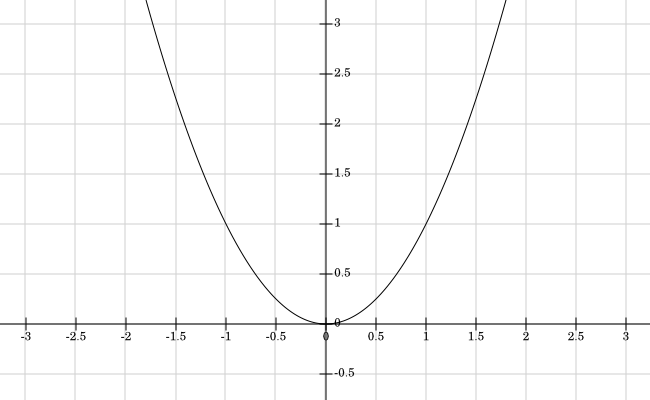
\includegraphics[width=0.7\textwidth]{assets/images/SHTIxCkjCR.png}
\end{figure}


The derivative of $y$ with respect to $x$ is obtained by replacing $x$ by a small change along that its direction $x \rightarrow x + \dot{x} \times o$, same for y with $y \rightarrow y + \dot{y} \times o$ and then :

\begin{equation*}
    \begin{split}
        y = x^2 & \leftrightarrow  (y + \dot{y} \times o) = (x + \dot{x} \times o)^2 \\
            & \leftrightarrow  (y + \dot{y} \times o) = x^2 +2x\dot{x}o + o^2 \\
            & \leftrightarrow  (y - x^2) + \dot{y} \times o = 2x\dot{x}o + o^2
    \end{split}
\end{equation*}

Since $y=x^2$, then :

$$
(y - x^2) + \dot{y} \times o = 2x\dot{x}o + o^2  \leftrightarrow \dot{y} \times o = 2x\dot{x}o + o^2 
$$

And because $o \neq 0$ : 


$$
\dot{y} = 2x\dot{x} + o
$$

And because $o$ is infinitesimally small we can ignore it. Then we end up with :

\begin{equation*}
    \begin{split}
        \dot{y} = 2x\dot{x} & \leftrightarrow \frac{\dot{y}}{\dot{x}} = 2x\\
                            & \leftrightarrow \frac{dy}{dx} = 2x\\
    \end{split}
\end{equation*}

Which is exactly what today we know being the derivative of $x^2$.

During the calculation of the derivative I used $\leftrightarrow$ instead of $\Leftrightarrow$. It's because at one point we say $o \neq 0$ to divide by $o$ and then later because $o$ is small we can ignore it (meaning $o=0$). That exactly what \href{https://en.wikipedia.org/wiki/History_of_calculus}{Leibniz blame Newton's theory} for the use of infinitesimally quantity. For more context see \href{https://en.wikipedia.org/wiki/Leibniz\%E2\%80\%93Newton_calculus_controversy}{Leibniz–Newton calculus controversy}). And that's also why today we are not making calculations with infinitesimally quantities ($dx$, $dy$, $d$t) as a part of the calculation (as "numbers"/objects like the other) but we use the notion of limits.

Nowadays we would have written :

\begin{equation*}
    \begin{split}
        \frac{dy}{dx} &= \alpha_{P_1} \\
                    &= \lim_{ h \to 0} \frac{f(x + h) - f(x)}{h} \\
                    & \underrel{h \to 0}{=} \frac{f(x + h) - f(x)}{h} + o(h)  \\
    \end{split}
\end{equation*}

Where $o(h)$ is the \href{https://simple.wikipedia.org/wiki/Big_O_notation}{Landau notation} (and not the Newton's $o$ notation).


\begin{equation*}
    \begin{split}
        \frac{dy}{dx} & \underrel{h \to 0}{=} \frac{f(x + h) - f(x)}{h} + o(h)  \\
                    &\Leftrightarrow f(x + h) \underrel{h \to 0}{=}  f(x) + \frac{dy}{dx} \times h - o(h) \\
                    &\Leftrightarrow  f(x + h) \underrel{h \to 0}{=} f(x) + \frac{dy}{dx} \times h + o(-h) \\
                    &\Leftrightarrow  f(x + h) \underrel{h \to 0}{=} f(x) + \frac{dy}{dx} \times h + o(h) \\
                    &\Leftrightarrow  f(x + h) \underrel{h \to 0}{=} f(x) + \frac{d}{dx}f \times h + o(h) \\
    \end{split}
\end{equation*}

Which is by the way the first order Taylor expansion of $f$.


%%%%%%%%%%%%%%%%%%%%%%%%%%%%%%%%%%%%%%%%%%%%%%%%%%%%%%%%%%%%%%%%
\subsubsection{Derivative computation}


Now, how computers compute derivatives numerically ? As we would do with any given graph, or experimentally : take a really small step in the input set of the function and use :

$$
\frac{f(x+h) - f(x)}{h} \approx f'(x) = \frac{df}{dx}
$$

Because $o(h)$ is so small, it can be ignored when $h \rightarrow 0$. Usually $h=10^{-6}$ in computer programs.

For example with $f: x \mapsto x^2$ the value of the derivative at the point $x=3$ with $h=10^{-6}$ is :

\begin{equation*}
    \begin{split}
        \frac{f(3+10^{-6})-f(3)}{10^{-6}} &= \frac{(3+10^{-6})^2 - 9}{10^{-6}}\\
            &= \frac{9,000006 - 9}{10^{-6}}\\
            &= \frac{0,000006}{10^{-6}}\\
            &= 6,000001 \\
            &\approx 2 \times 3 \\
    \end{split}
\end{equation*}

Then we need to do that for each desired point $x$

The main issue with this method is the precision of the result because some numbers \href{https://math.stackexchange.com/questions/943589/how-many-numbers-can-a-typical-computer-represent}{cannot} be represented exactly in computer, and there are some \href{https://docs.oracle.com/cd/E19957-01/806-3568/ncg_goldberg.html}{errors} which propagate in each operation made (rounding error, catastrophic cancellation, ...).
Theses issues are avoided by symbolic differentiation because there is no value at all, thus the computation is exact.


%%%%%%%%%%%%%%%%%%%%%%%%%%%%%%%%%%%%%%%%%%%%%%%%%%%%%%%%%%%%%%%%
%
%               AUTOMATIC DIFFERENTIATION
%
%%%%%%%%%%%%%%%%%%%%%%%%%%%%%%%%%%%%%%%%%%%%%%%%%%%%%%%%%%%%%%%%

\section{Automatic differentiation}

There is two modes of operation for AD : forward and backward modes.

%%%%%%%%%%%%%%%%%%%%%%%%%%%%%%%%%%%%%%%%%%%%%%%%%%%%%%%%%%%%%%%%
\subsection{Forward mode}

%%%%%%%%%%%%%%%%%%%%%%%%%%%%%%%%%%%%%%%%%%%%%%%%%%%%%%%%%%%%%%%%
\subsubsection{Integration of a function}

The integral of a function $f$ from $x_a \in Ker(f)$ to $x_b \in Ker(f)$, denoted $\int_{x_a}^{x_b} f(x)dx$, is by definition the area under that curve 

\begin{figure}[H]
 \centering
 \includesvg[width=0.7\columnwidth, svgpath = assets/images]{p49trQpD8i.svg}
\end{figure}

Here, $A := (x_a, y_a:=f(x_a))$ and $B := (x_b, y_b:=f(x_b))$

There are numerous definitions of integral but the simplest is the \href{https://en.wikipedia.org/wiki/Riemann_integral}{Riemann} one. The basic idea behind Riemann integral is to split the interval $[A, B]$ into small rectangles. If we split this interval into small enough rectangles then the sum will have as limits the area under the curve.

Let's take a look at a zoom of the graph of $f$ around the point $A$


\begin{figure}[H]
 \centering
 \includesvg[width=0.6\columnwidth, svgpath = assets/images]{dzs20Gp28G.svg}
\end{figure}

We approximate the area under $A$, $A'$ by the area of the rectangle with height $f(x_a)$. Then the area for that rectangle is : $f(x_a) \times (x_{a'} - x_a)$. We could also choose the bottom rectangle with height $f(x_a')$. In fact, the integrals are defined here as the unique limit of each upper and bottom rectangles sums.

%%%%%%%%%%%%%%%%%%%%%%%%%%%%%%%%%%%%%%%%%%%%%%%%%%%%%%%%%%%%%%%%
\subsubsection{Integral of derivative}

The \href{https://en.wikipedia.org/wiki/Fundamental_theorem_of_calculus}{fundamental theorem of calculus} (FTOC) give us : 
$$ \int_a^b (\frac{d}{dx}f)dx = f(b) - f(a) $$

Remember that the two $dx$ are quite not the same and we can not "simplify" by it. The $dx$ in the integral represents along which direction ($x$ axis) we integrate $f$.

But why is it true ?

Let's define $\mathcal{A}(x)_f$ the area of $f$ from $c \in Ker(f)$ as is the first defined value for $f$ with $c \geq 0$, to $x \in Ker(f)$. If $f$ is defined at $0$, then $c=0$. In other words, $\mathcal{A}(x)_f := \int_c^{x}f(x)dx$

As $A$ and $A'$ are really close, then, $A' := (x_a+h, f(x_a+h))$ with $h \neq 0$ and $(x+h) \in Ker(f)$.

The area from $A$ to $A'$ is then : $\mathcal{A}(x_a+h)_f - \mathcal{A}(x_a)_f$

$$ 
f(x_a +h) \times ( (x_a+h)-x_a) < \mathcal{A}(x_a+h)_f - \mathcal{A}(x_a)_f < f(x_a) \times ( x_a-(x_a+h))
$$

The left expression is the area defined by the upper rectangle and the right by the bottom one.

$$ 
f(x_a +h) \times h < \mathcal{A}(x_a+h)_f - \mathcal{A}(x_a)_f < f(x_a) \times h
$$

$h \neq 0$ :

$$ 
f(x_a +h) < \frac{\mathcal{A}(x_a+h)_f - \mathcal{A}(x_a)_f}{h} < f(x_a)
$$

When $h \rightarrow 0$ :

$$
\begin{cases}
f(x_a +h) \rightarrow f(x_a) \\
f(x_a) \rightarrow f(x_a) \\
\frac{\mathcal{A}(x_a+h)_f - \mathcal{A}(x_a)_f}{h} \rightarrow (\frac{d}{dx} \mathcal{A}(x)_f)|_{x=x_a}
\end{cases}
$$

Then,

$$ 
f(x_a) \leq  \big( \frac{d}{dx} \mathcal{A}(x)_f \big)|_{x=x_a} \leq f(x_a)
$$

Thus,

$$
\big( \frac{d}{dx} \mathcal{A}(x)_f \big)|_{x=x_a} = f(x_a)
$$

Since $x_a$ has been chosen arbitrarily, then :

$$
\frac{d}{dx} \mathcal{A}(x)_f = f
$$

With the usual notations, we have for $f$ continuous on $[a, x]$ :

$$
\begin{cases}
F(x) \mapsto \int_a^x f(x)dx \\
\frac{d}{dx}F = f
\end{cases}
$$

%%%%%%%%%%%%%%%%%%%%%%%%%%%%%%%%%%%%%%%%%%%%%%%%%%%%%%%%%%%%%%%%
\subsubsection{Taylor series}

For $f: \mathbb{C} \rightarrow \mathbb{R}$ infinitely differentiable at $a \in \mathbb{C}$ we have the following \href{https://en.wikipedia.org/wiki/Taylor_series}{Taylor power series} :

$$
f(x) = \sum_0^\infty  \frac{f^n(a)}{n!} (x-a)^n 
$$

where $f^n(a)$ denotes the n-th derivative of $f$ evaluated at the point $a$, and $f^0(a)=f(a)$.

An excellent proof is given \href{https://math.stackexchange.com/a/3261420/998679}{here}

%%%%%%%%%%%%%%%%%%%%%%%%%%%%%%%%%%%%%%%%%%%%%%%%%%%%%%%%%%%%%%%%
\subsubsection{Dual numbers}


\href{https://en.wikipedia.org/wiki/Dual_number}{Dual numbers} are the key to AD forward mode. A dual number is defined as a real part (called the primal part) and a dual part (called the tangent part) : 

$$
a + b\epsilon
$$

where :

$$
\begin{cases}
a,b \in \mathbb{R} \\
\epsilon \neq 0 \\
\epsilon^2 = 0
\end{cases}
$$


Dual numbers are part of the family of hyper-numbers as complex numbers are.
The definition of dual numbers can be quite out of context but as complex numbers, it has a history. To better understand how such numbers are discovered take a look at the excellent \href{https://www.youtube.com/watch?v=cUzklzVXJwo&ab_channel=Veritasium}{video} of {\it Veritasium}. And, to better understand how calculus is done with dual numbers take a look \href{https://www.youtube.com/watch?v=ceaNqdHdqtg&t=319s&ab_channel=MichaelPenn}{here}.

\href{https://math.stackexchange.com/questions/341535/is-the-theory-of-dual-numbers-strong-enough-to-develop-real-analysis-and-does-i}{History of dual numbers} can be linked to Newton calculus when in some calculations the term $dx^2$ was ignored (meaning $dx=0$) while $dx \neq 0$. 

So why dual numbers are useful for differentiation ?

Because for any function that admits a Taylor expansion, we have for $x=a+\epsilon$ where $a$ is the differentiable point of f :

\begin{equation*}
    \begin{split}
        f(x) = \sum_0^\infty  \frac{f^n(a)}{n!} (x-a)^n  &\Leftrightarrow \\
        f(a+\epsilon) = \sum_0^\infty  \frac{f^n(a)}{n!} (\epsilon)^n &\Leftrightarrow \\
        f(a+\epsilon) = f(a) + \frac{df}{dx}(a) \epsilon + \sum_2^\infty  \frac{f^n(a)}{n!} \epsilon^n
    \end{split}
\end{equation*}

Since for $n \geq 2$, $\epsilon^n = 0$, the :

$$
f(a+\epsilon) = f(a) + \frac{df}{dx}(a) \epsilon
$$

Thus, by computing the value of $f$ at $a+\epsilon$ we have the value of $f$ at $a$ and the exact value of the derivative of $f$ at $a$. This is not an approximation, but an exact value as if it was obtained with symbolic differentiation.

Denote that we can take a dual number as we can take complex number and use it as input for functions $\mathbf{R}^n \rightarrow \mathbf{R}^m$ since all usual operations in the rings $(\mathbf{R},+, \times)$ are defined (see \href{ttps://math.stackexchange.com/questions/464262/why-is-there-never-a-proof-that-extending-the-reals-to-the-complex-numbers-will}{1}, \href{https://www.arctbds.com/volume4/arctbds_submission_28.pdf}{2}). We just need to use a norm (which is a continuous function) when doing comparison.
For more exotic rings or operators we will need to define the use of dual number individually.

%%%%%%%%%%%%%%%%%%%%%%%%%%%%%%%%%%%%%%%%%%%%%%%%%%%%%%%%%%%%%%%%
\subsubsection{Gradient}

Let's focus on a more general case : multi-variable scalar function, also called scalar field function. As its name stands for, a multi-variable scalar function is a function $f : \mathbb{R}^n \rightarrow \mathbb{R}$ that takes as arguments variables $x$, $y$, $z$, ... and output a scalar in $\mathbb{R}$ or $\mathbb{C}$. For example the following function is a scalar field function :

$$
f : 
\begin{cases}
\mathbb{R} \rightarrow \mathbb{R} \\
(x, y) \mapsto \sin(x) \times y \\
\end{cases}
$$

Then to talks about derivatives we need to know on which variable we want to focus : $x$, $y$, $z$. In other words the single variable function derivatives case extends to multi-variable by taking the derivatives of the function for each variable. A derivative with respect to a variable is called a \href{https://en.wikipedia.org/wiki/Partial_derivative}{partial derivative} and usually denoted $\frac{\partial{f}}{\partial{x}}$, $\frac{\partial{f}}{\partial{y}}$, $\frac{\partial{f}}{\partial{z}}$, ...

Formally the directional derivative (if exists) is defined for $f$ at $a$ with respect to $x$ :

$$
\frac{\partial{f}}{x}(a_x, a_y, a_z, ...) = \lim_{ h \to 0} \frac{f(a_x+h, a_y, a_z, ...)-f(a_x, a_y, a_z, ...)}{h}
$$

Be aware that, having all well defined partial derivatives at $a$ does not mean the function is differentiable at that point ! If $f$ is continuous at $a$ then its differentiable at $a$. But $\text{continuous} \Rightarrow \text{differentiable}$ is given by another theorem and differentiation can be obtained without it (by the \href{https://en.wikipedia.org/wiki/Differentiable_function}{definition} for example, which imply the knowledge of topology).

We denote as \href{https://en.wikipedia.org/wiki/Gradient}{gradient} the vector of partial derivatives : $ \nabla f := (\frac{\partial{f}}{\partial{x}}, \frac{\partial{f}}{\partial{y}}, \frac{\partial{f}}{\partial{z}},...)$. It could be a line or a column vector and we go from one form to another with the \href{https://en.wikipedia.org/wiki/Transpose}{transpose} : 

$$
\begin{bmatrix}
    \frac{\partial{f}}{\partial{x}} \\
    \frac{\partial{f}}{\partial{y}} \\
    \frac{\partial{f}}{\partial{z}} \\
    \vdots \\
\end{bmatrix}^T = [\frac{\partial{f}}{\partial{x}}, \frac{\partial{f}}{\partial{y}}, \frac{\partial{f}}{\partial{z}},...]
$$

We usually talk about gradient for \href{https://en.wikipedia.org/wiki/Vector_spac}{vector spaces} when dealing with common functions. A vector space has a dimension denoted as $n$ which describes the number of possible directions along which we could move in that space and that define the space at the most elementary level. For example, $\mathbb{R}$ is a vector space of dimension 3 : $x$, $y$, $z$. We could also imagine a 4-th direction that makes a diagonal in the $x,y$ plan but then it would be a combination of the 3 previous directions. Since $x$, $y$, $z$ cannot be expressed as a combination of other elements in that space it's forming the axis/direction of the space. Together theses axis are forming a {\it family} of the vector space and are usually denotes as $(e_1, e_2, e_3, ...)$. 

Each element $a$ of the vector space can be written as a combination of a family of the vector space as $a = \sum_{i=1}^{n} a_i \times e_i$ with $a_i$ the coordinate of $a$ along the $e_i$ direction. For the common 2D and 3D vector space $(e_1, e_2, e_3)$ are denotes as $(\vec{i}, \vec{j}, \vec{k})$.

Since the $gradient$ is a vector we can express it through the axis of its living space as :

\begin{equation*}
[\frac{\partial{f}}{\partial{x}}, \frac{\partial{f}}{\partial{y}}, \frac{\partial{f}}{\partial{z}},...] 
\times
\begin{bmatrix}
    \vec{i} \\
    \vec{j} \\
    \vec{k} \\
    \vdots \\
\end{bmatrix}
= \frac{\partial{f}}{\partial{x}}\vec{i} + \frac{\partial{f}}{\partial{y}}\vec{j} + \frac{\partial{f}}{\partial{z}}\vec{k} + ...
\end{equation*}

And abusively we just write $\frac{\partial{f}}{\partial{x}} + \frac{\partial{f}}{\partial{y}} + \frac{\partial{f}}{\partial{z}}$. But the gradient is not a scalar !


%%%%%%%%%%%%%%%%%%%%%%%%%%%%%%%%%%%%%%%%%%%%%%%%%%%%%%%%%%%%%%%%
\subsubsection{Directional derivative}

If the partial derivative of a function represents the rate of change of that function along the corresponding direction, then the \href{https://www.youtube.com/watch?v=N_ZRcLheNv0&ab_channel=KhanAcademy}{directional derivative} represents the rate of change of the function along an arbitrary chosen direction.

For 
$v= \in \begin{bmatrix}
    v_x \\
    v_y \\
    v_z \\
    \vdots \\
\end{bmatrix} \mathbb{R}^n$ 
the directional derivative of $f$ for any $a \in \mathbb{R}^n$ is :

$$
\nabla_{v}f(a) = \lim_{h \rightarrow 0} \frac{f(a+hv)-f(a)}{h}
$$

with $h$ a scalar

\href{ttps://en.wikipedia.org/wiki/Directional_derivative}{And}, $\nabla_{v}f(a) = v \times \nabla f(a)$

Here, the directional derivative is a scalar which is the sum of all partial derivative with respect to each axis defined by the directional vector $v$ (it's a dot product - the multiplication operator extension to vector).

$$
v \times \nabla f(a) = v_x \times \frac{\partial{f}}{\partial{x}}(a) + v_y \times \frac{\partial{f}}{\partial{y}}(a) + v_z \times \frac{\partial{f}}{\partial{z}}(a) 
$$

%%%%%%%%%%%%%%%%%%%%%%%%%%%%%%%%%%%%%%%%%%%%%%%%%%%%%%%%%%%%%%%%
\subsubsection{Jacobian}

The gradient is in fact a particular case of the \href{https://en.wikipedia.org/wiki/Jacobian_matrix_and_determinant}{Jacobian}. The Jacobian is the same thing as the gradient but defined for function with multiple output values $f : \mathbb{R}^n \rightarrow \mathbb{R}^m$. Such a function is decomposed for each coordinate of the output as a new function :

$$
f : 
\begin{cases}
\mathbb{R}^n \rightarrow \mathbb{R}^m \\
\begin{bmatrix}
    x_1 \\
    x_2 \\
    \vdots \\
    x_n
\end{bmatrix} \mapsto

\begin{bmatrix}
    f_1(x_1, x_2, ..., x_n) \\
    f_2(x_1, x_2, ..., x_n) \\
    \vdots \\
    f_m(x_1, x_2, ..., x_n) \\
\end{bmatrix}

\end{cases}
$$

For example $f$ can be :

$$
f : (x,y) \mapsto (x \times y, \cos(x))
$$

And if you think of $f$ as the application of a single variable function ($\sin$ for example) to a vector, we get a vector as the output that also can be described as different functions :

$$
f : 
\begin{bmatrix}
    x \\
    y \\
\end{bmatrix}
 \mapsto \sin \big(
    \begin{bmatrix}
    x \\
    y \\
    \end{bmatrix}
 \big) = \begin{bmatrix}
    \sin(x) \\
    \sin(y) \\
\end{bmatrix}
:= \begin{bmatrix}
    f_1(x, y) \\
    f_2(x, y) \\
\end{bmatrix}
$$

In fact, all functions than we can think of are built in the scenario of single variable function and then generalized for multi-variable function usually by applying that function for each component. 

The Jacobian of a multi-variable function is then :

$$
\begin{bmatrix}
    \frac{\partial{f_1}}{x_1}(x_1, x_2, ..., x_n) & \frac{\partial{f_1}}{x_2}(x_1, x_2, ..., x_n)  & ... & \frac{\partial{f_1}}{x_n}(x_1, x_2, ..., x_n) \\

    \vdots & \vdots & \vdots & \vdots \\

    \frac{\partial{f_m}}{x_1}(x_1, x_2, ..., x_n) & \frac{\partial{f_m}}{x_2}(x_1, x_2, ..., x_n)  & ...  &\frac{\partial{f_m}}{x_n}(x_1, x_2, ..., x_n) \\
\end{bmatrix}
$$

Now let's extend the Taylor series for scalar field functions. Let's define $f : \mathbb{R}^n \rightarrow \mathbb{R}$ a scalar field function.

Remember that the goal is the get the Taylor expansion for scalar field functions to extend the use of dual numbers to such functions. In fact, we just need to get the expansion to the order 2 as seen previously. In fact, there is a complete formula of the Taylor series for multi-variable functions but it comes without real context :


\begin{figure}[H]
\centering
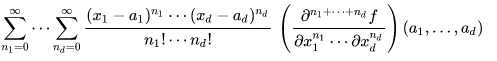
\includegraphics[width=0.7\textwidth]{assets/images/Dx93rZHiBg.png}
\end{figure}


The proof previously made with integral could possibly also be done like that, but we would need to use \href{https://en.wikipedia.org/wiki/Line_integral}{lines integral} (used for integral of multi-variable functions) which is really more complex to manipulate.

In fact, there is \href{https://math.stackexchange.com/questions/221669/derivation-of-multivariable-taylor-series}{more elegant and simple proof} at least for our use case.

Let's consider $f$ a $C^2$ scalar field function ($f$ is continuous and its derivatives up to the order 2 are continuous). The proof could be made with less powerful hypotheses but will be harder to write and understand.

The directional derivative of $f$ in the direction defined by $a \in \mathbb{R}^n$ at $r \in \mathbb{R}^n$ arbitrary chosen is :

$$
a \times \nabla f(r) = \lim_{h \rightarrow 0} \frac{f(r+ha)-f(r)}{h}
$$

Now let's consider :
$
g : \begin{cases}
\mathbb{R} \rightarrow \mathbb{R} \\
h \mapsto f(r+ha)
\end{cases}
$

$g$ is a single variable function (since $r$ and $a$ are fixed). The only changing par is $h$. And since $f$ is a scalar field, then $f(r+ah) \in \mathbb{R}$.

Let's suppose that $f$ is 2-differentiable ($f$ admits at least derivatives of the order 2 at $r$). Then $f$ is continuous at $0$, thus $g$ is continuous at $0$ and admits derivative of the order 2.

Then, since $g$ is a 1-dimensional function we can use the Taylor series expansion for any $h \in \mathbb{R}$ :

$$
g(h) = g(0) + g'(0)h + \frac{1}{2}g''(0)h^2 + \mathbf{o}(h^2)
$$

- 
$$
g(0) = f(r+a \times 0) = f(r)
$$
- for $x \in \mathbb{R}$ arbitrary chosen (and since $f$ is continuous) :

\begin{equation*}
    \begin{split}
        g'(x) &= \lim_{l \rightarrow 0} \frac{g(x+l)-g(x)}{l} \\
        &=  \lim_{l \rightarrow 0} \frac{f(r+(x+l)a)-f(r+xa)}{l} \\
    \end{split}
\end{equation*}

Let's consider $X := r+xa$, then

\begin{itemize}

\item
    \begin{equation*}
        \begin{split}
            g'(x) &= \lim_{l \rightarrow 0} \frac{f(X+la)-f(X)}{l} \\
            &=  \nabla_{a} f(X) \\
            &=  \nabla_{a} f(r+xa) \\
        \end{split}
    \end{equation*}
    
\item
    $$
    g'(0) = \nabla_{a} f(r+0 \times a) =  \nabla_{a} f(r) = a \nabla f(r)
    $$

\item

    \begin{equation*}
        \begin{split}
            g''(0) &= \lim_{l \rightarrow 0} \frac{g'(0+l)-g'(0)}{l} \\
            &= \lim_{l \rightarrow 0} \frac{\nabla_{a} f(r+la)-\nabla_{a} f(r)}{l} \\
        \end{split}
    \end{equation*}

\end{itemize}

Let's consider 
$
\phi : \begin{cases}
\mathbb{R}^n \rightarrow \mathbb{R} \\
x \mapsto \nabla_{a} f(x)
\end{cases}
$

Since the directional derivative is a linear combination of the partial derivatives and since $f$ is $\mathbb{C}^2$, then $\nabla_{a} f$ is differentiable and continuous. Thus, 

\begin{equation*}
    \begin{split}
    g''(0) &= \lim_{l \rightarrow 0} \frac{\phi(r+la)-\phi(r)}{l} \\
    &= \nabla_{a} \phi(r) \\
    \end{split}
\end{equation*}

$g''(0)$ is the directional derivative of the directional derivative of $f$ at $r$ along the direction of $a$. It's denoted as $\nabla_{a}^2 f(r)$ or $\nabla_{a} \nabla_{a} f(r)$.

Then,

\begin{equation*}
    \begin{split}
        g(h) = f(r) + \nabla_{a}f(r)h + \nabla_{a}^2 f(r)h^2 + \mathbf{o}(h^2) &\Leftrightarrow \\
        f(r+ha) = f(r) + \nabla_{a}f(r)h +  \nabla_{a}^2 f(r)h^2 + \mathbf{o}(h^2) \\
    \end{split}
\end{equation*}

Since $r$, $a$, $h$ were arbitrary chosen, thus for $h=0+\epsilon$ :

$$
f(r+a \epsilon) = f(r) + \nabla_{a}f(r)\epsilon + 0
$$

Thus, the dual number "trick" can also be applied to scalar field functions. For $i \in [1...n]$ (in integer interval from $1$ to $n$) and 
$
a = \begin{bmatrix}
\delta_{i, 1} \\
\delta_{i, 2} \\
\vdots \\
\delta_{i, i} \\
\vdots \\
\delta_{i, n}
\end{bmatrix}
$, we get :

$$
f(r+a \epsilon) = f(r) + \frac{\partial{f}}{\partial{x_i}}\epsilon
$$

where $x_i$ is the i-th variable of the function $f$ and $\delta{i, j}$ the  Kronecker's delta ($1$ if $i=j$, else $0$).

Finally, for multi-variable functions we need to compute each partial derivative through the use of dual number.


%%%%%%%%%%%%%%%%%%%%%%%%%%%%%%%%%%%%%%%%%%%%%%%%%%%%%%%%%%%%%%%%
\subsubsection{Hessian}

For $f: \mathbb{R}^n \rightarrow \mathbb{R}$ the Taylor expansion at $a \in \mathbb{R}$ for $x \in \mathbb{R}^n$ is  :

$$
f(x) = f(a) + \nabla f(a)(x-a) + \frac{1}{2}(x-a)^T Hf(a)(x-a) + \mathbf{o}((x-a)^2)
$$

where $Df$ is the gradient of $f$ and $Hf$ the hessian of $f$ (which is the "derivative" of the order 2 of $f$)

$$
Hf= \begin{bmatrix}
\frac{\partial^2{f}}{\partial{x_1}^2} & \frac{\partial^2{f}}{\partial{x_1}\partial{x_2}} & ... & \frac{\partial^2{f}}{\partial{x_1}\partial{x_n}} \\

\frac{\partial^2{f}}{\partial{x_2}\partial{x_1}} & \frac{\partial^2{f}}{\partial{x_2}^2} & ... & \frac{\partial^2{f}}{\partial{x_2}\partial{x_n}} \\

\vdots & \vdots & \vdots & \vdots \\

\frac{\partial^2{f}}{\partial{x_n}\partial{x_n}} & \frac{\partial^2{f}}{\partial{x_n}\partial{x_n}} & ... & \frac{\partial^2{f}}{\partial{x_n}^2} \\

\end{bmatrix}
$$

For 
$
f: \begin{cases}
\mathbb{R}^n \rightarrow \mathbb{R}^m \\
x \mapsto (f_1(x), f_2(x), ..., f_m(x))
\end{cases}
$ the hessian is : $Hf = (Hf_1, Hf_2, ..., Hf_m)$ a \href{https://en.wikipedia.org/wiki/Tensor}{tensor}. A tensor is a n-dimensional structure that holds data and adapts it to the transformation of the surrounding space where the tensor live. For example, with a tensor no matter how the usual 3D space coordinate system is oriented, rotated, translated, the tensor will represent the same thing by adapting its inner values according to the transformation of its surrounding space. So it's not just a matrix (see \href{https://www.youtube.com/watch?v=bpG3gqDM80w&ab_channel=TheScienceAsylum}{1}, \href{ttps://medium.com/@quantumsteinke/whats-the-difference-between-a-matrix-and-a-tensor-4505fbdc576c}{2}).

\href{https://math.stackexchange.com/questions/1822100/how-to-do-a-taylor-expansion-of-a-vector-valued-function}{Here} is an example of such a hessian.


%%%%%%%%%%%%%%%%%%%%%%%%%%%%%%%%%%%%%%%%%%%%%%%%%%%%%%%%%%%%%%%%
\subsubsection{Matrix}

For $f: \mathbb{R}^{n \times m} \rightarrow \mathbb{R}^{p \times q}$ function of matrices things get more complicated for the Taylor series since the multiplication of matrix is not commutative. 

However, the Taylor series can be generalized to many other objects (see \href{https://math.stackexchange.com/questions/4177818/taylor-series-coordinate-free-form/4177847#4177847}{1}, \href{https://math.stackexchange.com/questions/3271948/proving-limit-of-fx-tnfx-taylor-is-zero-in-multivariable-calculus/3272515#3272515}{2}).


%%%%%%%%%%%%%%%%%%%%%%%%%%%%%%%%%%%%%%%%%%%%%%%%%%%%%%%%%%%%%%%%
\subsubsection{Implementation}

Finally, the AD forward mode uses dual numbers to get one by one the partial derivatives. This is can be achieved in programs by overloading operators and function in the programming language.

\begin{lstlisting}[language=Python, escapeinside={(*}{*)}, numbers=none]
class DualNumber:
    def __init__(self, primal, tangent=1):
        self.primal = primal # real part
        self.tangent = tangent # dual part
    
    def __add__(self, v):
        # right addition : current_object + input object
        if type(v) is DualNumber:
            return DualNumber(self.primal+v.primal, self.tangent+v.tangent)
        else: # scalar addition
            return DualNumber(self.primal+v, self.tangent)
    
    ...
\end{lstlisting}

Then, we need to define functions for dual numbers as well  : 


\begin{lstlisting}[language=Python, escapeinside={(*}{*)}, numbers=none]
def sin(input_value):
    if type(input_value) is DualNumber:
        return DualNumber(math.sin(input_value.primal), input_value.tangent*math.cos(input_value.primal))
    
    return math.sin(input_value)
\end{lstlisting}


This mode of AD works well when the number of inputs is smaller than the number of outputs because we need to do the computation as many times as there is inputs (with the previous example one with $(a_1 + \epsilon, a_2)$ and two with $(a_1, a_2+\epsilon)$). When the number of outputs is greater than the one of the input we use another method: the backward mode.


%%%%%%%%%%%%%%%%%%%%%%%%%%%%%%%%%%%%%%%%%%%%%%%%%%%%%%%%%%%%%%%%
\subsection{Backward mode}

The forward mode was the more complex in math because we needed to make sure to understand how we can obtain exact derivative. The backward mode is in fact really simple and straightforward but the catch is in the implementation which is trickier. 

%%%%%%%%%%%%%%%%%%%%%%%%%%%%%%%%%%%%%%%%%%%%%%%%%%%%%%%%%%%%%%%%
%%%%%%%%%%%%%%%%%%%%%%%%%%%%%%%%%%%%%%%%%%%%%%%%%%%%%%%%%%%%%%%%
%%%%%%%%%%%%%%%%%%%%%%%%%%%%%%%%%%%%%%%%%%%%%%%%%%%%%%%%%%%%%%%%
%%%%%%%%%%%%%%%%%%%%%%%%%%%%%%%%%%%%%%%%%%%%%%%%%%%%%%%%%%%%%%%%
%%%%%%%%%%%%%%%%%%%%%%%%%%%%%%%%%%%%%%%%%%%%%%%%%%%%%%%%%%%%%%%%
\iffalse

\begin{figure}[H]
\centering
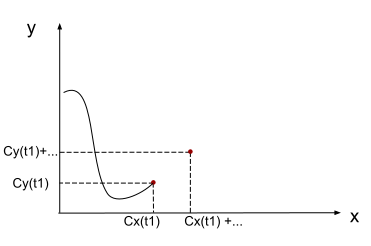
\includegraphics[width=0.2\textwidth]{assets/images/sQ6Rxqpqbe.svg}
\end{figure}


\begin{figure}[H]
 \centering
 \includesvg[width=0.7\columnwidth, svgpath = assets/images]{yQAOsqOt4J.svg}
\end{figure}

\fi


\end{document}
